\documentclass[11pt]{article}
\usepackage{fontspec}
\usepackage{amsmath}
\usepackage{unicode-math}
\setmainfont{TeX Gyre Pagella}
\setmathfont{TeX Gyre Pagella Math}
\setsansfont{TeX Gyre Heros}[Scale=0.92]
\setmonofont{TeX Gyre Cursor}[Scale=0.90]
\usepackage[a4paper,margin=2.3cm]{geometry}
\usepackage{xcolor}
\usepackage{titlesec}
\usepackage{enumitem}
\usepackage{booktabs}
\usepackage{tabularx}
\usepackage{caption}
\usepackage{tikz}
\usetikzlibrary{arrows.meta,positioning,calc,patterns,decorations.pathreplacing,fit,backgrounds}
\usepackage[european,RPvoltages]{circuitikz}
\usepackage[hidelinks]{hyperref}

\definecolor{ink}{RGB}{20,22,28}
\definecolor{grey}{RGB}{110,118,130}
\definecolor{hi}{RGB}{20,90,170}
\color{ink}

\captionsetup{font=small,labelfont=bf,labelsep=period}
\renewcommand{\figurename}{Rys.}
\renewcommand{\tablename}{Tab.}
\renewcommand{\contentsname}{Spis treści}

\titleformat{\section}{\Large\bfseries\sffamily}{\thesection.}{0.5em}{}
\titleformat{\subsection}{\large\bfseries\sffamily}{\thesubsection.}{0.5em}{}
\titlespacing*{\section}{0pt}{1.2em}{0.4em}
\titlespacing*{\subsection}{0pt}{0.8em}{0.2em}
\setlength{\parindent}{0pt}\setlength{\parskip}{0.5em}
\setlist[itemize]{leftmargin=1.4em,itemsep=0.15em,topsep=0.2em}

\begin{document}

\begin{center}
{\sffamily\bfseries\LARGE Wyjaśnienia techniczne}\\[3pt]
{\sffamily\large Control Pilot, front-end, przekaźniki, moc, zabezpieczenia, układy N/PE/PEN}\\[5pt]
{\color{grey}\rule{0.8\linewidth}{0.8pt}}\\[3pt]
{\sffamily\small Dawid Cekała \quad$\cdot$\quad przygotowanie do pracy w AMPERE POINT}
\end{center}
\vspace{0.5em}
{\small\tableofcontents}
\newpage

% ===================================================================
\section{Sygnał Control Pilot: jak powstaje, jak wygląda, jak go odczytać}

Control Pilot (CP) to pojedyncza żyła sygnałowa w złączu Type~2, którą ładowarka i pojazd uzgadniają ładowanie. To samo zachowanie sygnału tłumaczy, dlaczego multimetr pokazał stany skupione powyżej 9~V zamiast tablicowych 12/9/6/3~V.

\subsection{Tor sygnału}

Sygnał przechodzi przez kilka ogniw (Rys.~\ref{fig:tor}). Mikrokontroler wytwarza logiczny przebieg prostokątny 1~kHz na poziomie 0--3{,}3~V. Sam w sobie nie nadaje się na linię, bo CP wymaga $\pm12$~V. Dlatego trafia do układu pośredniczącego (front-end nadawczy), który wzmacnia go do $\pm12$~V i podaje na linię przez rezystor szeregowy $R_1=1\ \mathrm{k\Omega}$. Po stronie pojazdu dioda i rezystory (2{,}74~k$\Omega$, dołączany 1{,}3~k$\Omega$) ściągają dodatni szczyt do poziomu danego stanu. Z powrotem do mikrokontrolera napięcie wraca przez front-end odbiorczy (dzielnik i układ ograniczający), który sprowadza $\pm12$~V do bezpiecznego okna przetwornika analogowo-cyfrowego.

\begin{figure}[h]\centering
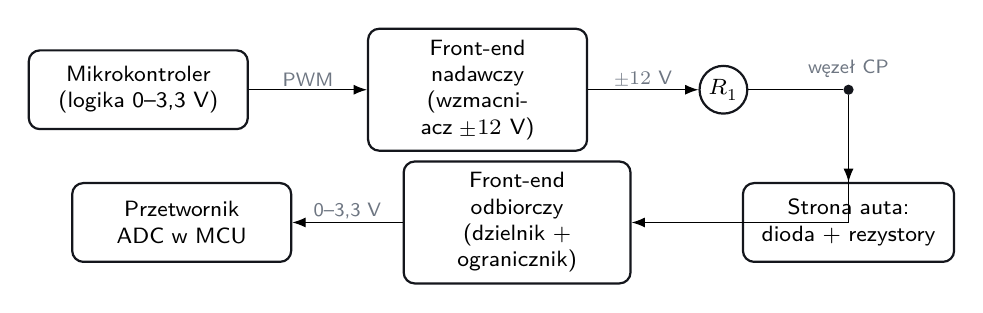
\begin{tikzpicture}[font=\sffamily\footnotesize,>=Latex,
 b/.style={draw=ink,thick,rounded corners,align=center,inner sep=4pt,minimum height=1cm,text width=2.5cm},
 n/.style={font=\sffamily\scriptsize,color=grey,inner sep=1pt}]
 \node[b](mcu){Mikrokontroler\\(logika 0--3{,}3~V)};
 \node[b,right=1.5cm of mcu](tx){Front-end\\nadawczy\\(wzmacniacz $\pm12$~V)};
 \node[draw=ink,thick,circle,right=1.4cm of tx,inner sep=1.5pt](r1){$R_1$};
 \node[circle,fill=ink,inner sep=1.3pt,right=1.2cm of r1](cp){};
 \node[above=1pt of cp,n]{węzeł CP};
 \node[b,below=1.1cm of cp,text width=2.4cm](car){Strona auta:\\dioda + rezystory};
 \node[b,left=1.4cm of car,text width=2.6cm](rx){Front-end\\odbiorczy\\(dzielnik + ogranicznik)};
 \node[b,left=1.4cm of rx](adc){Przetwornik\\ADC w MCU};
 \draw[->](mcu)--(tx) node[midway,above,n]{PWM};
 \draw[->](tx)--(r1) node[midway,above,n]{$\pm12$~V};
 \draw[-](r1)--(cp);
 \draw[->](cp)--(car) node[midway,right,n]{};
 \draw[->](cp) |- (rx);
 \draw[->](rx)--(adc) node[midway,above,n]{0--3{,}3~V};
\end{tikzpicture}
\caption{Tor sygnału CP: mikrokontroler $\to$ front-end nadawczy $\to$ $R_1$ $\to$ węzeł CP $\to$ front-end odbiorczy $\to$ ADC. Front-end to dwa układy pośredniczące: jeden tworzy $\pm12$~V, drugi sprowadza je do okna ADC.}
\label{fig:tor}
\end{figure}

\subsection{Jak wygląda przebieg}

W stanie spoczynku (A) ładowarka jeszcze nie nadaje modulacji --- CP to stałe $+12$~V. Gdy pojawia się pojazd, ładowarka włącza falę prostokątną 1~kHz: górą $+12$~V, dołem $-12$~V. Strona auta ściąga \emph{dodatni szczyt} do poziomu stanu: około $+9$~V (B, podłączony) albo $+6$~V (C, ładowanie). Dół zostaje na $-12$~V --- to kontrola obecności diody. Szerokość górnej części, czyli \emph{wypełnienie}, koduje oferowany prąd (Rys.~\ref{fig:cp}).

\begin{figure}[h]\centering
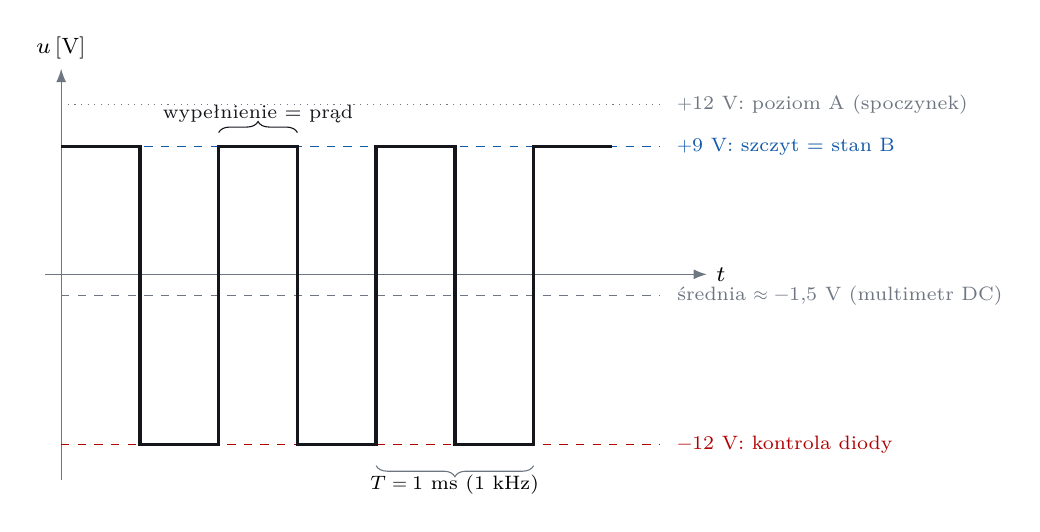
\begin{tikzpicture}[font=\sffamily\footnotesize,>=Latex,xscale=1.0,yscale=0.9]
 % axes
 \draw[->,grey] (-0.2,0)--(8.2,0) node[right,black]{\(t\)};
 \draw[->,grey] (0,-2.9)--(0,2.9) node[above,black]{\(u\,[\mathrm{V}]\)};
 % reference dashed levels
 \draw[dashed,hi] (0,1.8)--(7.6,1.8);
 \draw[dashed,red!70!black] (0,-2.4)--(7.6,-2.4);
 \draw[dashed,grey] (0,-0.3)--(7.6,-0.3);
 \draw[dotted,grey] (0,2.4)--(7.6,2.4);
 % square wave B: high +9 (1.8), low -12 (-2.4), period 2, duty 0.5, 3 periods
 \draw[very thick,ink]
   (0,1.8)--(1,1.8)--(1,-2.4)--(2,-2.4)--(2,1.8)--(3,1.8)--(3,-2.4)--(4,-2.4)--(4,1.8)--(5,1.8)--(5,-2.4)--(6,-2.4)--(6,1.8)--(7,1.8);
 % labels
 \node[hi,anchor=west,font=\scriptsize] at (7.7,1.8) {\(+9\) V: szczyt = stan B};
 \node[red!70!black,anchor=west,font=\scriptsize] at (7.7,-2.4) {\(-12\) V: kontrola diody};
 \node[grey,anchor=west,font=\scriptsize] at (7.7,-0.3) {średnia \(\approx -1{,}5\) V (multimetr DC)};
 \node[grey,anchor=west,font=\scriptsize] at (7.7,2.4) {\(+12\) V: poziom A (spoczynek)};
 % duty brace
 \draw[decorate,decoration={brace,amplitude=4pt},ink] (2,2.0)--(3,2.0) node[midway,above,font=\scriptsize]{wypełnienie = prąd};
 % period brace
 \draw[decorate,decoration={brace,mirror,amplitude=4pt},grey] (4,-2.7)--(6,-2.7) node[midway,below,font=\scriptsize,black]{\(T=1\) ms (1 kHz)};
\end{tikzpicture}
\caption{Przebieg CP w stanie B (wypełnienie 50\% dla czytelności). Stan określa \textbf{dodatni szczyt} ($+9$~V), nie wartość średnia. Multimetr DC pokazuje średnią ($\approx -1{,}5$~V), a w trybie AC wartość skuteczną ($\approx 10{,}6$~V) --- żadna z nich nie równa się $9$~V.}
\label{fig:cp}
\end{figure}

\subsection{Jak czyta to układ ładowarki}

Mikrokontroler próbkuje CP \emph{w rytm własnego PWM}: raz w fazie wysokiej (łapie dodatni szczyt $\to$ stan), raz w fazie niskiej (sprawdza $-12$~V $\to$ dioda). To celowane próbkowanie w znanym momencie, więc układ odczytuje prawdziwe poziomy 12/9/6/3~V.

\subsection{Jak czyta to multimetr (i dlaczego wyszło dziwnie)}

Multimetr nie próbkuje „w szczycie''. W trybie napięcia stałego pokazuje wartość średnią całej fali, a w trybie zmiennego --- wartość skuteczną. Dla fali o dodatnim szczycie $V_p$, dole $-12$~V i wypełnieniu $D$:
\begin{align}
U_{\text{śr}} &= V_p\,D + (-12)\,(1-D),\\
U_{\text{rms}} &= \sqrt{V_p^{2}\,D + 12^{2}\,(1-D)}.
\end{align}
Dla stanu B ($V_p=9$~V, $D=0{,}5$): $U_{\text{śr}}=-1{,}5$~V, $U_{\text{rms}}\approx 10{,}6$~V. Kluczowe jest to, że przy małym wypełnieniu (mały oferowany prąd) dominuje dół $-12$~V, obecny przez większość okresu. Wtedy wartość skuteczna dla wszystkich stanów skupia się blisko $11$--$12$~V i różni się tylko nieznacznie --- dokładnie to zmierzyłeś (wszystko powyżej 9~V, różnice rzędu miliwoltów). Stan A wyszedł poprawnie, bo tam CP to czyste $+12$~V stałe. Wniosek: multimetr pokazuje uśrednioną mieszankę, a nie poziom stanu. To artefakt pomiaru, nie usterka.

\subsection{Jak czyta to oscyloskop}

Oscyloskop rysuje napięcie w czasie, więc widzisz wprost: poziomy $\pm12$~V, ściągnięty dodatni szczyt (9/6/3~V = stan), okres 1~ms i wypełnienie (= prąd). To jedyny prosty przyrząd, który odczytuje stan CP poprawnie. Stąd zasada: do CP bierz oscyloskop, nie multimetr.

% ===================================================================
\section{Front-end --- co to dokładnie jest}

„Front-end'' to analogowy układ pośredniczący między cyfrowym mikrokontrolerem a rzeczywistym sygnałem. Mikrokontroler pracuje na małych napięciach logicznych (0--3{,}3~V) i nie może ani wytworzyć $\pm12$~V, ani bezpiecznie zmierzyć takiego napięcia. Front-end załatwia obie te rzeczy (Rys.~\ref{fig:fe}).

\begin{itemize}
 \item \textbf{Strona nadawcza.} Logiczny przebieg PWM z mikrokontrolera trafia na wzmacniacz operacyjny zasilany z $+12$ i $-12$~V. Wzmacniacz przerzuca wyjście między $+12$ a $-12$~V w rytm PWM i podaje sygnał na linię przez $R_1=1\ \mathrm{k\Omega}$. To z tego powstaje fala CP.
 \item \textbf{Strona odbiorcza.} Węzeł CP zmienia się w zakresie $\pm12$~V --- to za dużo dla wejścia ADC. Dzielnik rezystorowy skaluje napięcie do okna 0--3{,}3~V, a diody ograniczające (do masy i do $+3{,}3$~V) chronią wejście przed przepięciem. Tak przygotowane napięcie czyta przetwornik.
\end{itemize}

\begin{figure}[h]\centering
\begin{circuitikz}[european,font=\sffamily\footnotesize,scale=0.92,transform shape]
 % transmit op-amp
 \node[op amp,scale=0.8](OA){};
 \node[left=0.1cm of OA.+,font=\scriptsize,align=right](in){PWM\\z MCU};
 \draw(in.east)--(OA.+);
 \draw(OA.-) -- ++(0,-0.6) -| (OA.out);
 \node[above,font=\scriptsize] at (OA.up){$+12$};
 \node[below,font=\scriptsize] at (OA.down){$-12$};
 \draw(OA.out) to[R,l_=$R_1{=}1\,\mathrm{k\Omega}$] ++(3,0) coordinate(cp);
 \node[circle,fill=ink,inner sep=1.2pt] at (cp){};
 \node[above,font=\scriptsize] at (cp){węzeł CP};
 \draw(cp) -- ++(1,0) node[right,font=\scriptsize]{do auta};
 % receive divider + clamp
 \draw(cp) -- ++(0,-1.4) coordinate(a) to[R,l_=$R_a$] ++(0,-1.4) coordinate(b);
 \node[circle,fill=ink,inner sep=1.2pt] at (b){};
 \draw(b) to[R,l_=$R_b$] ++(0,-1.4) node[ground]{};
 \draw(b) -- ++(2,0) node[right,font=\scriptsize](adc){do ADC};
 % clamp diodes
 \draw(b) ++(1,0) coordinate(cl) to[D,l=\,] ++(0,1.2) node[above,font=\scriptsize]{$+3{,}3$~V};
 \draw(cl) to[D,*-] ++(0,-1.2) node[ground]{};
\end{circuitikz}
\caption{Front-end CP. U góry: wzmacniacz operacyjny zasilany $\pm12$~V tworzy falę i podaje ją przez $R_1$. U dołu: dzielnik $R_a/R_b$ i diody ograniczające sprowadzają napięcie węzła CP do bezpiecznego okna 0--3{,}3~V przetwornika ADC.}
\label{fig:fe}
\end{figure}

% ===================================================================
\section{Przekaźnik, stycznik i skąd sześć sztuk}

Przekaźnik i stycznik działają tak samo: cewka elektromagnesu przyciąga zworę, która zwiera lub rozwiera styki. Różnica jest klasy, nie zasady. Stycznik to przekaźnik mocy --- większy prąd, kilka biegunów głównych, gaszenie łuku, wytrzymałość na wiele łączeń; przekaźnik to ogólniejszy, zwykle mniejszy łącznik. Czyli stycznik to „ciężki'' przekaźnik do toru mocy.

Dlaczego więc sześć sztuk, skoro jeden stycznik ma 3--4 bieguny? Bo to, co widziałeś, to najpewniej \emph{sześć pojedynczych przekaźników}, a nie sześć wielobiegunowych styczników. W ładowarkach AC (zwłaszcza OEM) zamiast jednego stycznika z połączonymi biegunami często stosuje się bank pojedynczych przekaźników --- po jednym na przewód. Instalacja 3-fazowa ma L1, L2, L3 i N, czyli \textbf{cztery} przewody do przełączenia. Pozostałe dwa to zwykle (Rys.~\ref{fig:rel}):

\begin{itemize}
 \item drugi łącznik w szeregu na wybranych przewodach --- \textbf{podwójne przerwanie}: gdy jeden styk się sklei, drugi i tak odcina (wymóg pewnego rozłączania), albo
 \item osobne odłączanie przewodu neutralnego przy ochronie przed zanikiem PEN (patrz rozdz.~\ref{sec:pen}).
\end{itemize}

Dokładny podział potwierdzisz, śledząc płytkę: które przekaźniki są w szeregu na tym samym przewodzie (redundancja), a które po jednym na fazę. Liczba 6 to nie „sześć styczników po 4 bieguny'', tylko sześć pojedynczych łączników na przewodach i w torach redundantnych.

\begin{figure}[h]\centering
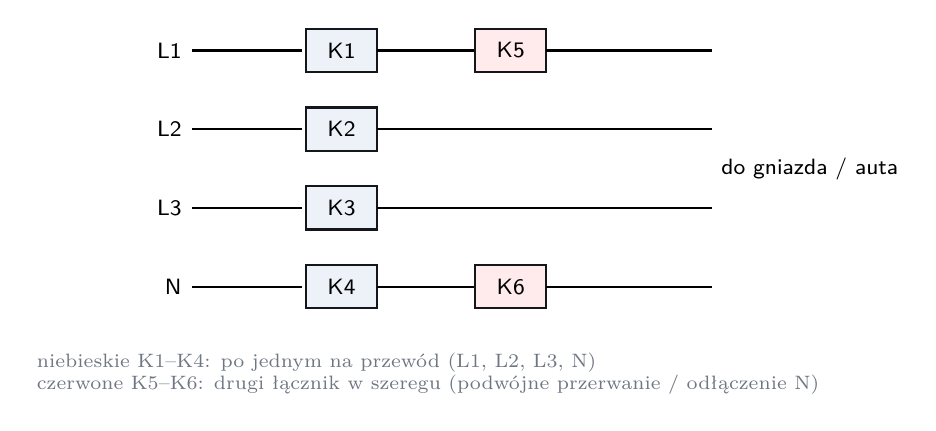
\begin{tikzpicture}[font=\sffamily\footnotesize,
 k/.style={draw=ink,thick,fill=hi!8,minimum width=0.9cm,minimum height=0.55cm,inner sep=1pt},
 k2/.style={draw=ink,thick,fill=red!8,minimum width=0.9cm,minimum height=0.55cm,inner sep=1pt}]
 \foreach \y/\name in {3/L1,2/L2,1/L3,0/N}{
   \draw[thick] (0,\y) node[left]{\name} -- (1.4,\y);
   \draw[thick] (5.3,\y) -- (6.6,\y);
 }
 \node[k] at (1.9,3){K1}; \node[k] at (1.9,2){K2}; \node[k] at (1.9,1){K3}; \node[k] at (1.9,0){K4};
 \draw[thick](2.35,3)--(3.6,3); \draw[thick](2.35,2)--(5.3,2); \draw[thick](2.35,1)--(5.3,1); \draw[thick](2.35,0)--(3.6,0);
 \node[k2] at (4.05,3){K5}; \node[k2] at (4.05,0){K6};
 \draw[thick](4.5,3)--(5.3,3); \draw[thick](4.5,0)--(5.3,0);
 \node[right] at (6.6,1.5){do gniazda / auta};
 \node[align=left,font=\scriptsize,color=grey] at (3.0,-1.1){niebieskie K1--K4: po jednym na przewód (L1, L2, L3, N)\\czerwone K5--K6: drugi łącznik w szeregu (podwójne przerwanie / odłączenie N)};
\end{tikzpicture}
\caption{Sześć pojedynczych przekaźników: cztery na przewody (L1, L2, L3, N) i dwa w szeregu na wybranych torach (redundancja lub odłączanie N). To nie to samo, co jeden stycznik o czterech biegunach.}
\label{fig:rel}
\end{figure}

% ===================================================================
\section{Prąd a moc (P35 vs P72)}

Obie ładowarki są jednofazowe, więc moc to po prostu \(P=U\cdot I\) przy \(U=230\)~V:
\[
P_{35}=230\cdot 16 \approx 3{,}68\ \mathrm{kW},\qquad
P_{72}=230\cdot 32 \approx 7{,}36\ \mathrm{kW}.
\]
Dwa razy większy prąd to dwa razy większa moc --- skaluje się wprost. Wrażenie, że „nie wychodzi podwójnie'', bierze się tylko z zaokrągleń w katalogu (ta sama wartość 7{,}36~kW bywa zapisywana raz jako 7{,}2, raz jako 7{,}4~kW).

Moc przestaje być wprost proporcjonalna do prądu dopiero, gdy zmienia się coś \emph{poza} prądem: napięcie, liczba faz albo współczynnik mocy. Dla trzech faz \(P=3\,U\,I\). Stąd P11 ma ten sam prąd 16~A co P35, ale 11~kW zamiast 3{,}7~kW --- dodatkowa moc bierze się z trzech faz, a nie z większego prądu:
\[
P_{11}=3\cdot 230\cdot 16 \approx 11\ \mathrm{kW}.
\]

% ===================================================================
\section{Matematyka: napięcie, prąd, moc, energia}

\subsection{Definicje i jednostki}
\begin{itemize}
 \item Prąd to przepływ ładunku w czasie: \( i=\dfrac{dq}{dt}\); jednostka amper, \(\mathrm{A=C/s}\).
 \item Napięcie to energia na jednostkę ładunku: \( u=\dfrac{dW}{dq}\); jednostka wolt, \(\mathrm{V=J/C}\).
 \item Moc chwilowa: \( p(t)=u(t)\,i(t)\); jednostka wat, \(\mathrm{W=V\cdot A}\).
 \item Energia to całka mocy po czasie: \( E=\displaystyle\int_0^T p(t)\,dt\); jednostka dżul, \(\mathrm{J=W\cdot s}\). W rozliczeniach \(1~\mathrm{kWh}=3{,}6~\mathrm{MJ}\), więc \( E[\mathrm{kWh}]=\dfrac{1}{3{,}6\cdot10^{6}}\displaystyle\int p\,dt\).
\end{itemize}

\subsection{Wartość średnia, skuteczna i PWM}
Wartość średnia i skuteczna przebiegu w okresie \(T\):
\[
\langle x\rangle=\frac1T\int_0^T x\,dt,\qquad
X_{\mathrm{rms}}=\sqrt{\frac1T\int_0^T x^2\,dt}.
\]
Moc na rezystancji zależy od kwadratu, więc od wartości skutecznej: \(P=U_{\mathrm{rms}}^2/R=U_{\mathrm{rms}}I_{\mathrm{rms}}\). W sieci AC: \(P=U\,I\cos\varphi\) (wartości skuteczne, \(\cos\varphi\) = współczynnik mocy). Fala prostokątna o poziomach \(0\) i \(V\) oraz wypełnieniu \(D\) ma wartość średnią \(\langle x\rangle = V\cdot D\) --- to jest istota kodowania PWM: wypełnienie niesie wartość, a uśrednienie (filtr lub całkowanie) ją odzyskuje.

\subsection{Układy, które to realizują}
\begin{itemize}
 \item \textbf{Pomiar prądu}: bocznik (z prawa Ohma \(u=R\,i\), mierzysz spadek napięcia) albo czujnik Halla (bezstykowo, z pola magnetycznego). \textbf{Pomiar napięcia}: dzielnik rezystorowy.
 \item \textbf{Mnożenie} \(u\cdot i\): układ mnożący albo mikrokontroler próbkujący \(u\) i \(i\) przetwornikiem i mnożący je cyfrowo.
 \item \textbf{Całkowanie} (energia): integrator na wzmacniaczu operacyjnym (Rys.~\ref{fig:int}) daje \( v_{out}=-\frac{1}{RC}\int v_{in}\,dt\); cyfrowo to sumowanie próbek mocy. Niezerowalny licznik energii to dedykowany układ liczący \(\int u\,i\,dt\) i wystawiający impulsy (stała liczba impulsów na kWh).
\end{itemize}

\begin{figure}[h]\centering
\begin{circuitikz}[european,font=\sffamily\footnotesize,scale=0.9,transform shape]
 \node[op amp,scale=0.8](A){};
 \draw (A.-) -- ++(-0.6,0) coordinate(m) to[R,l=$R$] ++(-1.8,0) node[left]{$v_{in}$};
 \draw (A.+) -- ++(-0.6,0) node[ground]{};
 \draw (m) -- ++(0,1.1) to[C,l=$C$] ++(1.9,0) -| (A.out);
 \draw (A.out) -- ++(0.5,0) node[right]{$v_{out}$};
\end{circuitikz}
\caption{Integrator na wzmacniaczu operacyjnym: napięcie wyjściowe jest proporcjonalne do całki wejścia. Tak realizuje się sumowanie energii w czasie.}
\label{fig:int}
\end{figure}

% ===================================================================
\section{Zabezpieczenia: na nadmiar czego działają i jak wpięte}

Każde zabezpieczenie reaguje na inną wielkość i jest inaczej włączone w obwód (Tab.~\ref{tab:prot}, Rys.~\ref{fig:prot}).

\begin{table}[h]\centering\small
\begin{tabularx}{\linewidth}{@{}l X l l@{}}
\toprule
\textbf{Zabezpieczenie} & \textbf{Reaguje na} & \textbf{Wpięcie} & \textbf{Kod} \\
\midrule
Nadprądowe / zwarcie & nadmiar prądu w torze & szeregowo & B, F \\
Różnicowoprądowe (RCD + 6\,mA DC) & prąd upływu (różnica L--N) & obejmująco & G \\
Przepięciowe / podnapięciowe & napięcie poza zakresem & pomiarowo & C, D \\
Przegrzanie & nadmiar temperatury & czujnik & A \\
Uziemienie / PE & brak lub błąd PE, zamiana L--N & monitoring PE & E \\
\bottomrule
\end{tabularx}
\caption{Zabezpieczenia serii P i sposób ich działania.}
\label{tab:prot}
\end{table}

\begin{figure}[h]\centering
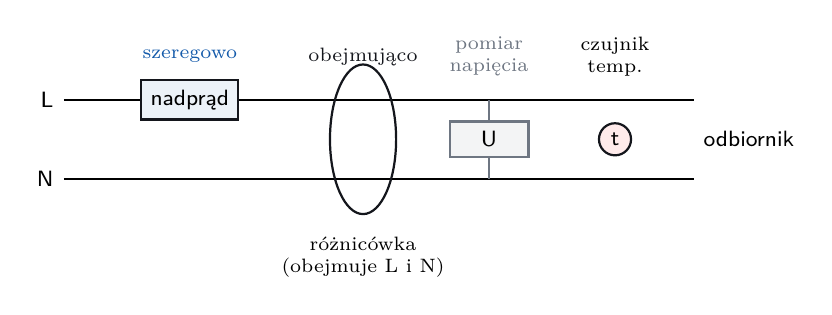
\begin{tikzpicture}[font=\sffamily\footnotesize,>=Latex]
 \draw[thick] (0,1) node[left]{L} -- (8,1);
 \draw[thick] (0,0) node[left]{N} -- (8,0);
 % series overcurrent on L
 \node[draw=ink,thick,fill=hi!8,minimum width=1.2cm,minimum height=0.5cm] at (1.6,1){nadprąd};
 % RCD toroid encircling both
 \draw[thick,ink] (3.8,0.5) ellipse (0.42 and 0.95);
 \node[align=center,font=\scriptsize] at (3.8,-1.0){różnicówka\\(obejmuje L i N)};
 % voltage measure tap
 \draw[thick,grey] (5.4,1)--(5.4,0.6) node[midway,right,font=\scriptsize]{};
 \draw[thick,grey] (5.4,0.6)--(5.4,0.4); \draw[thick,grey](5.4,0.4)--(5.4,0);
 \node[draw=grey,thick,fill=grey!8,minimum width=1.0cm,minimum height=0.45cm] at (5.4,0.5){U};
 \node[font=\scriptsize,grey,align=center] at (5.4,1.55){pomiar\\napięcia};
 % temp sensor near load
 \node[draw=ink,thick,fill=red!8,circle,inner sep=1.5pt] at (7.0,0.5){\,t\,};
 \node[font=\scriptsize,align=center] at (7.0,1.55){czujnik\\temp.};
 \node[right] at (8,0.5){odbiornik};
 \node[left,align=right] at (0,-0.0){};
 % wiring style labels
 \node[font=\scriptsize,hi] at (1.6,1.55){szeregowo};
 \node[font=\scriptsize,ink] at (3.8,1.55){obejmująco};
\end{tikzpicture}
\caption{Trzy sposoby wpięcia: szeregowo (nadprądowe --- przerywa tor), obejmująco (różnicówka --- mierzy różnicę prądów L i N), pomiarowo (napięcie, temperatura --- mierzą, nie przerywają same z siebie).}
\label{fig:prot}
\end{figure}

% ===================================================================
\section{Przewód neutralny (N), ochronny (PE) i ochronno-neutralny (PEN)}\label{sec:pen}

W instalacji występują przewody o różnych rolach (Rys.~\ref{fig:tn}):
\begin{itemize}
 \item \textbf{Neutralny (N)} --- roboczy. Prowadzi prąd powrotny odbiornika (w układzie 3-fazowym prąd nierównowagi). Ponieważ płynie nim prąd, ma spadek napięcia \(u=i\,Z\), więc jego potencjał nie jest dokładnie zerem ziemi i nieco rośnie pod obciążeniem.
 \item \textbf{Ochronny (PE)} --- bezpieczeństwa. Normalnie nie płynie nim prąd, więc jego potencjał jest praktycznie równy ziemi na całej długości. Łączy metalowe obudowy z ziemią i daje drogę prądowi zwarcia, co wyzwala zabezpieczenie.
 \item \textbf{Ochronno-neutralny (PEN)} --- jeden przewód łączący obie role (układ TN-C). Tym samym przewodem płynie prąd roboczy i jest on zarazem odniesieniem ochronnym. Problem: skoro płynie prąd, jest spadek napięcia, więc obudowy podpięte do PEN nie są dokładnie na potencjale ziemi. A jeśli PEN się przerwie, obudowy mogą znaleźć się pod napięciem fazowym --- realne zagrożenie.
\end{itemize}

Dlatego nowoczesne instalacje rozdzielają PEN na osobne PE i N (TN-S, albo TN-C-S z rozdziałem w rozdzielnicy), a do odbiorników --- w tym ładowarek EV --- prowadzi się osobny, pewny PE. Ładowarka wymaga poprawnego PE i go monitoruje (błąd E), bo użytkownik dotyka nadwozia auta. W instalacjach TN-C-S stosuje się też wykrywanie zaniku PEN --- i to jest jeden z powodów dodatkowych przekaźników z rozdz.~3.

\begin{figure}[h]\centering
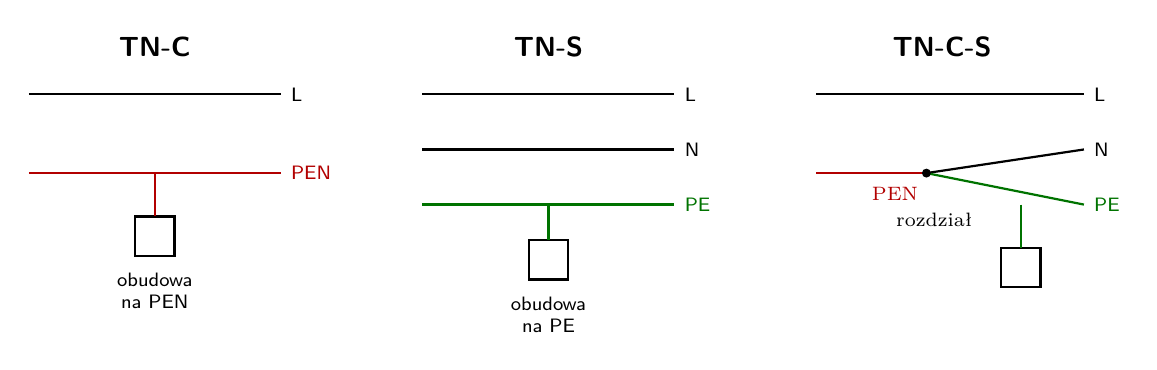
\begin{tikzpicture}[font=\sffamily\scriptsize,>=Latex]
 \foreach \x/\t in {0/{TN-C}, 5/{TN-S}, 10/{TN-C-S}}{
   \node[font=\sffamily\bfseries] at (\x+1.6,2.6){\t};
 }
 % TN-C
 \draw[thick](0,2)--(3.2,2) node[right]{L}; 
 \draw[thick,red!70!black](0,1)--(3.2,1) node[right]{PEN};
 \node[draw,thick,minimum size=0.5cm] at (1.6,0.2){\,}; \draw[thick,red!70!black](1.6,1)--(1.6,0.45);
 \node[align=center] at (1.6,-0.5){obudowa\\na PEN};
 % TN-S
 \draw[thick](5,2)--(8.2,2) node[right]{L};
 \draw[thick](5,1.3)--(8.2,1.3) node[right]{N};
 \draw[thick,green!45!black](5,0.6)--(8.2,0.6) node[right]{PE};
 \node[draw,thick,minimum size=0.5cm] at (6.6,-0.1){\,}; \draw[thick,green!45!black](6.6,0.6)--(6.6,0.15);
 \node[align=center] at (6.6,-0.8){obudowa\\na PE};
 % TN-C-S
 \draw[thick](10,2)--(13.4,2) node[right]{L};
 \draw[thick,red!70!black](10,1)--(11.4,1) coordinate(split);
 \draw[thick](11.4,1)--(13.4,1.3) node[right]{N};
 \draw[thick,green!45!black](11.4,1)--(13.4,0.6) node[right]{PE};
 \filldraw (11.4,1) circle(1.4pt); \node[below,font=\scriptsize,red!70!black] at (11.0,0.95){PEN};
 \node[font=\scriptsize] at (11.5,0.4){rozdział};
 \node[draw,thick,minimum size=0.5cm] at (12.6,-0.2){\,}; \draw[thick,green!45!black](12.6,0.6)--(12.6,0.05);
\end{tikzpicture}
\caption{TN-C: wspólny PEN (roboczy i ochronny w jednym --- ryzykowny). TN-S: osobne N i PE. TN-C-S: PEN rozdzielany w jednym punkcie na N i PE; dalej do odbiornika idą osobne przewody. Ładowarki EV wymagają osobnego, pewnego PE.}
\label{fig:tn}
\end{figure}

\end{document}
